\documentclass[a4paper,12pt]{article}
\usepackage{graphicx}
\usepackage{listings}
\usepackage{amsmath}
\usepackage{color}
\usepackage{titlesec}


\begin{document}
\title{Conditional Analysis}
\author{Martin Moran}
\maketitle

\section*{Conditional Analysis}
Finding a pair of SNPs which have a high pairwise IHS does not necessarily mean that they are being positively selected. The location of SNPs can effect their IHS. If a nearby SNP is being positively selected it can cause SNPs physically near that locus to appear to be positively selected for. It is assumed that a single SNP is more likely to be positively selected for than a pair of SNPs. In this case we must conditionally analyse the SNP pairs to see if it is being affected by the the nearby SNPs. 

\begin{figure}[h!]
  \centering
    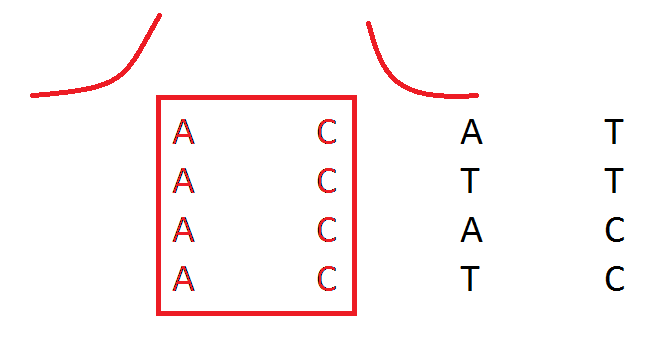
\includegraphics[scale=0.5]{conditional1}
  \caption{Pairwise IHS of first and second SNP}
\end{figure}

We begin by performing the pairwise IHS for a pair of alleles, as shown in figure 1. If we find that this is a high IHS we must investigate nearby single SNPs for their effect on the pair of SNPs. We find the IHS for SNPs within a certain distance of the pairwise IHS as shown in figure 2.

\begin{figure}[h!]
  \centering
    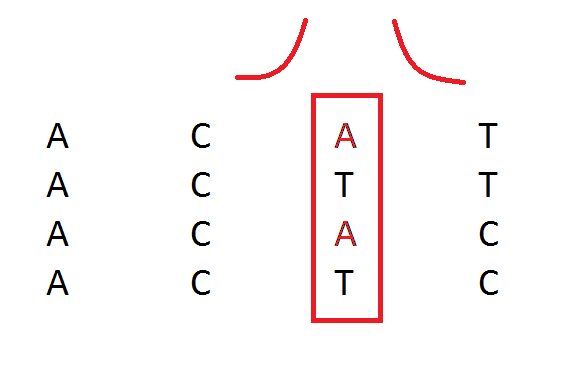
\includegraphics[scale=0.5]{conditional2}
  \caption{IHS of third SNP}
\end{figure}

\newpage
We precondition the pair of SNPs with respect to these single SNPs. This means we find the IHH of the original pair of SNPs who also have the allele of the single SNP which we have found to have high IHS as shown in figure 3. We also find the IHS for the pair without this SNP. If we find that the IHH of the the preconditioned pair with the SNP is similar to the IHH without the SNP we can deduce that the pair of SNPs are being positively selected independently of that SNP. If it is higher we can deduce that the locality of the pair of SNPs to the positively selected SNP is causing the high pairwise IHS.

\begin{figure}[h!]
  \centering
    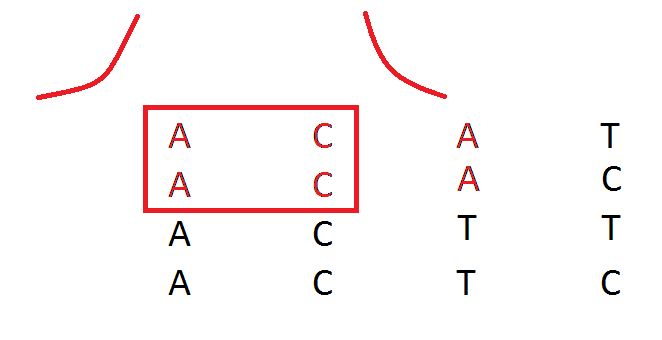
\includegraphics[scale=0.5]{conditional4}
  \caption{Pairwise IHH of first and second SNP preconditioned  with respect to A in the third SNP}
\end{figure}

[I am aware that I need a better way of representing IHS and IHH, as currently it confuses the imagery with EHH]
\end{document}